\section{نتیجه‌گیری}
در پایان این فصل روشن شد که رادارهای \lr{FMCW} با بهره‌گیری از سیگنال‌های \lr{Chirp} و تحلیل \lr{Range–Doppler} می‌توانند حرکات بسیار کوچک ناشی از ضربان قلب را با دقت میلی‌متری تشخیص دهند. افزایش پهنای باند و طول چرخه مدولاسیون (\lr{Tp}) به‌طور مستقیم دقت فاصله‌سنجی را بهبود می‌بخشد، در حالی که حفظ نسبت سیگنال به نویز (\lr{SNR}) بالا برای جداسازی ضربان از نویز محیطی و حرکات تصادفی بدن حیاتی است.

پیشرفت‌های اخیر در پردازش دوبعدی \lr{Range–Doppler} \cite{neemat2019reconfigurable} و نمونه‌برداری انتخابی \cite{kwak2024adjusting} دامنه سرعت قابل اندازه‌گیری را گسترش داده و امکان پایش ضربان قلب در شرایط محیطی و سوژه‌های متحرک بیشتر را فراهم کرده‌اند. روش‌های کاهش نویز مبتنی بر تجزیه مقادیر منفرد (\lr{SVD}) \cite{lv2024millimeter} و بررسی اثرات تغییرات درون‌فردی سیگنال‌های \lr{seismocardiogram} \cite{demirsoy2024investigating} نیز دقت تخمین نرخ ضربان و \lr{HRV} را ارتقاء داده‌اند.

علاوه بر این، کاربرد رادار میلی‌متری در پایش چندسوژه‌ای \cite{islam2020non} و تشخیص چندهدفه \lr{HRV} \cite{xu2024health} نشان داده که با طراحی مناسب آنتن و الگوریتم‌های هوشمند، می‌توان به راه‌حل‌های غیرتماسی دقیق و کارآمد برای کاربردهای پزشکی دست یافت. با این وجود، چالش‌هایی نظیر تداخل متقابل میان سوژه‌ها، کاهش \lr{SNR} در محیط‌های شلوغ و پیچیدگی محاسباتی پردازش \lr{Range–Doppler} همچنان باقی است.

\begin{figure}[ht]
    \centering
    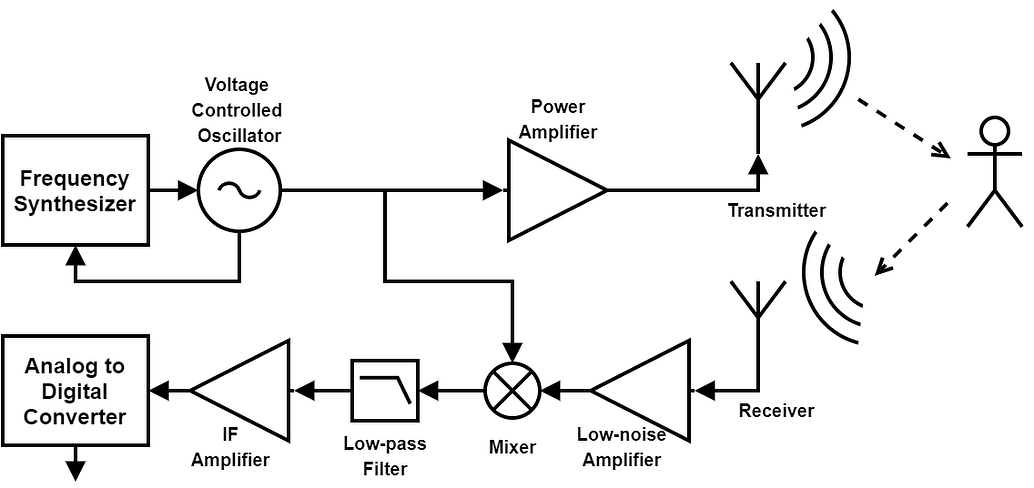
\includegraphics[width=0.7\linewidth]{Images/chapter2/2-3.png}
    \caption{اندازه‌گیری علائم حیاتی با استفاده از رادار \lr{mmWave FMCW} \cite{digikey_fmcw}.}
    \label{fig:fmcw_vitals}
\end{figure}

\vspace{5cm}

فصل بعدی با تکیه بر این مبانی، روش پیشنهادی پژوهش را تشریح خواهد کرد، که در آن با طراحی آزمایش و انتخاب پارامترهای بهینه رادار، تلاش می‌شود محدودیت‌های مطرح‌شده برطرف گردد و کارایی سیستم در پایش ضربان قلب واقعی ارزیابی شود.


